\chapter{Serving Layer: API and Dashboard}
\label{chap:serving-layer}

\providecommand{\servingcell}[1]{\begin{minipage}[t]{\linewidth}#1\end{minipage}}
\providecolor{cmdcolor}{RGB}{0,92,160}
\providecommand{\tablehead}[1]{\textcolor{cmdcolor}{\textbf{#1}}}

\section{Role of the Serving Layer}

The serving layer is the user access point of RAPID. Its role is not to recompute the indicators produced by the batch and speed layers. Rather, it makes these results queryable through a Web interface and homogeneous JSON responses. In the project's Lambda Architecture, it therefore connects three elements: the historical views stored in HBase, the real-time results stored in Cassandra, and the HTML/JavaScript dashboard that presents this information to the analyst.

This layer exposes the results through the Flask API hosted at \texttt{http://100.73.216.115:5000}. The frontend does not read HBase or Cassandra directly. It only consumes the REST endpoints defined in the service contract, then transforms JSON responses into summary cards, charts, tables, alert feeds and detail windows. This choice keeps the interface decoupled from internal storage details: the dashboard does not need to know the Cassandra queries, HBase scans, or Spark processing that produced the views.

The serving layer therefore addresses two complementary needs. First, it allows users to consult historical batch views from HBase: IP reputation, attack patterns, threat timeline, volumes, port scans and multi-step attacks. Second, it exposes recent operational results from Cassandra: threat scores, signature alerts, volume alerts, real-time threats, adaptive threshold and attack map. The user obtains a unified view without directly seeing the storage difference between the two temporalities.

\section{Dashboard Architecture}

The \texttt{dashboard/} folder contains a static interface composed of HTML, CSS and JavaScript files. The \texttt{index.html} file automatically redirects to \texttt{batch.html}, making the batch view the current entry page. The real-time view remains available through \texttt{dashboard.html}. Both pages share the same general logic. A top bar displays the RAPID identity, the API connection status, the clock and the refresh indication. A control bar then enables IP address search, polling pause, manual refresh and JSON export. The main content is organized into cards, charts and tables.

The \texttt{batch.html} view is HBase-oriented. It contains tab navigation: \textit{Overview}, \textit{Attack Patterns}, \textit{IP Reputation}, \textit{Port Scans} and \textit{Multi-Step}. The page first presents KPI cards to count attack patterns, flagged IPs, port scans, multi-step chains, threat volumes and available HBase tables. The tabs then provide access to historical charts and detailed tables.

Figure~\ref{fig:batch-dashboard-overview-timeline} illustrates the main batch dashboard view, where the analyst verifies the HBase status, historical indicators and temporal evolution of threats.

\begin{figure}[H]
    \centering
    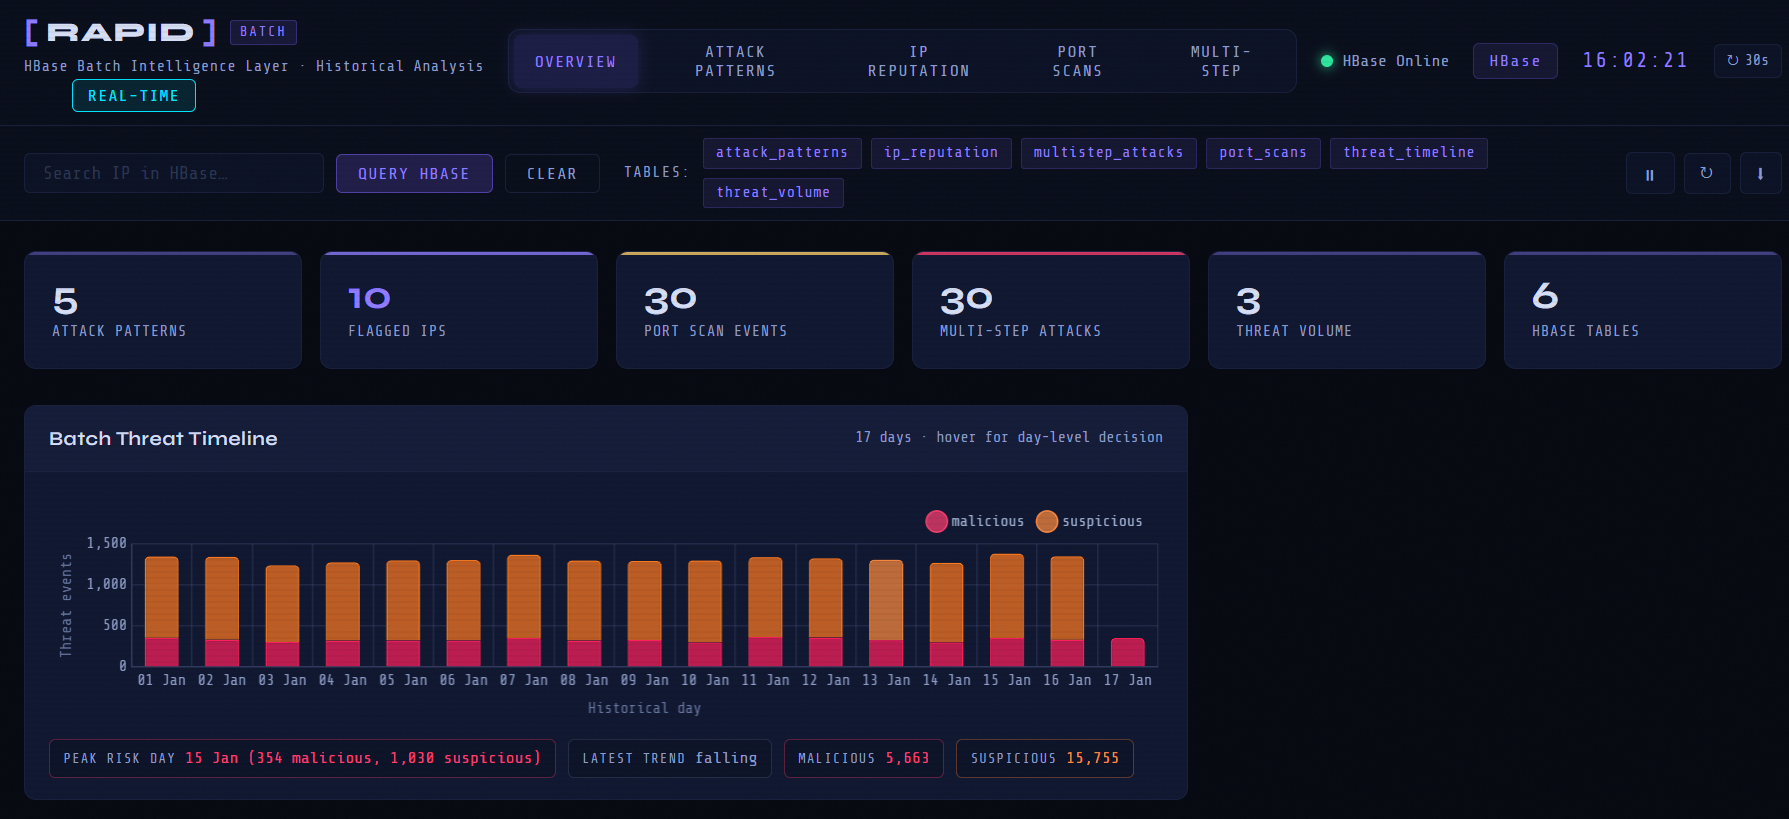
\includegraphics[width=\textwidth]{figures/serving/batch_dashboard/batch_dashboard_overview_timeline.png}
    \caption{General view of the RAPID batch dashboard displaying the HBase status, historical indicators and threat timeline.}
    \label{fig:batch-dashboard-overview-timeline}
\end{figure}

The \texttt{dashboard.html} view is oriented toward the speed layer. It displays real-time scores, volume alerts, signature alerts, a real-time decision queue, an activity timeline and a D3.js attack map. It also contains an IP search modal window that queries the \texttt{/threats/ip/<ip>} endpoint in order to display the score, threat level, recommendation, historical score and associated alerts.

Figure~\ref{fig:speed-dashboard-overview} illustrates the upper part of the real-time view, where the analyst visualizes the main indicators, the maximum score and the distribution of detections.

\begin{figure}[H]
    \centering
    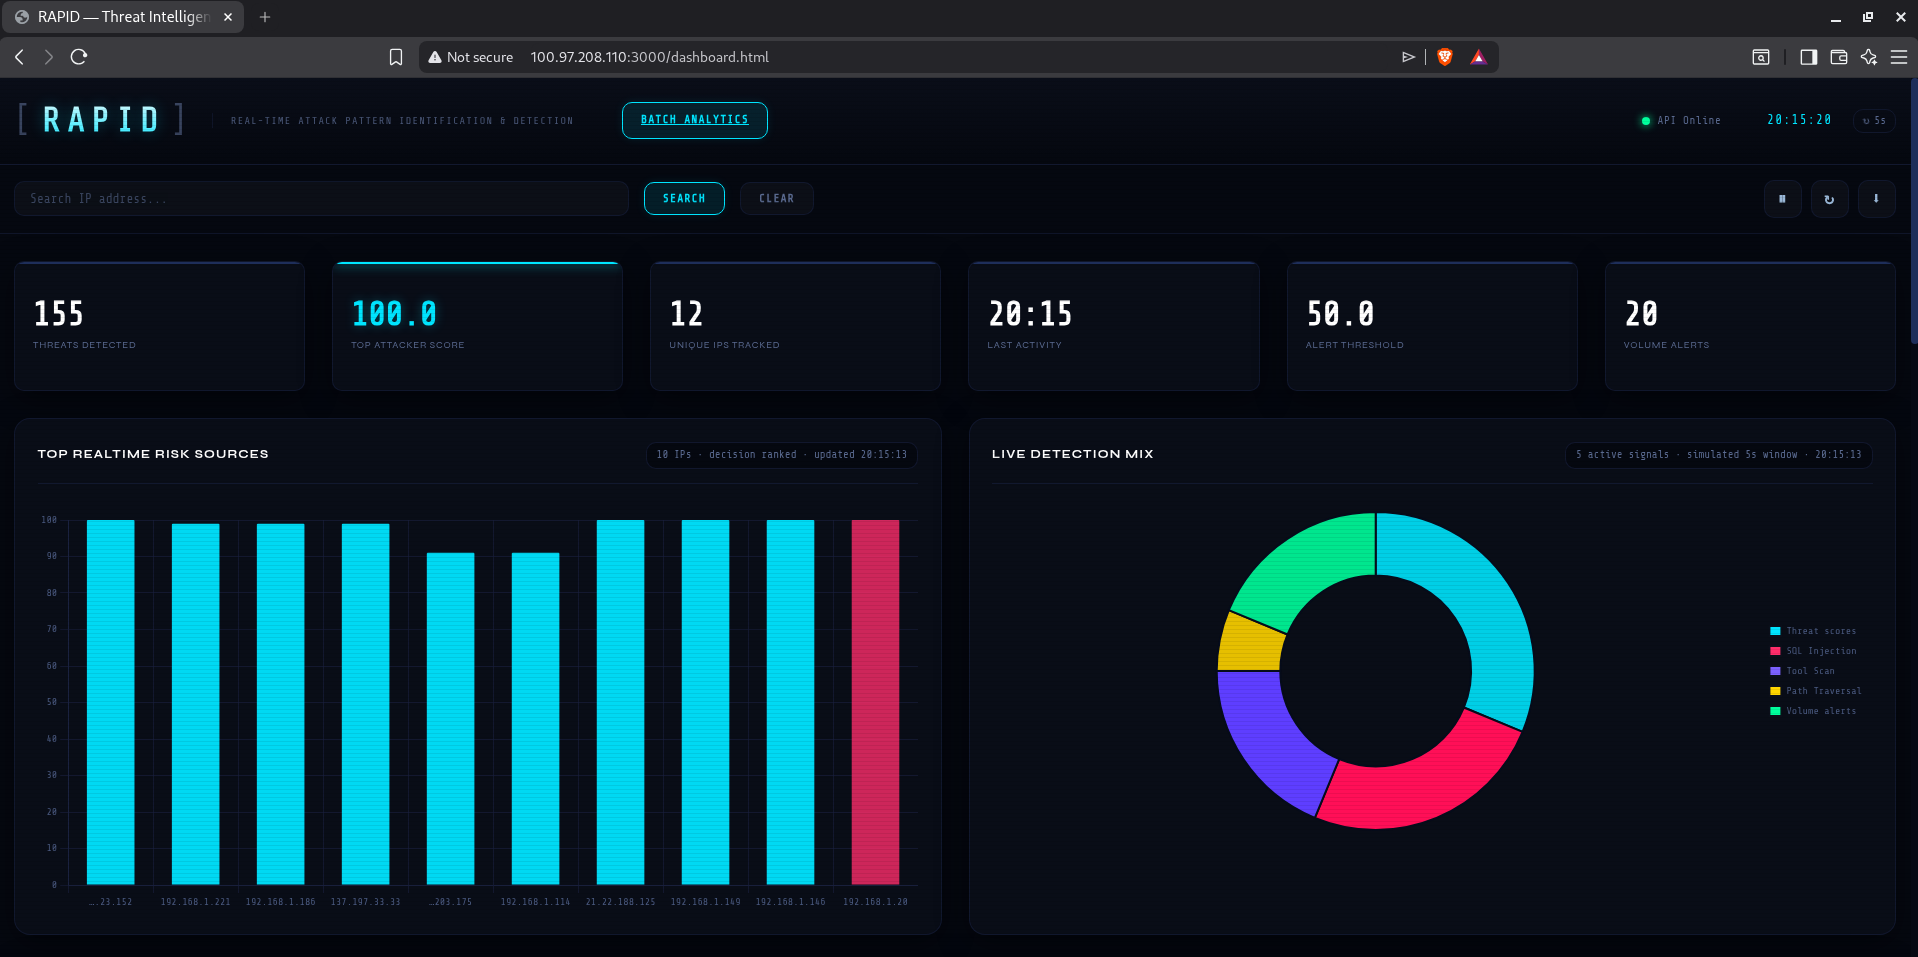
\includegraphics[width=\textwidth]{figures/serving/speed_dashboard/speed_dashboard_overview_top.png}
    \caption{General view of the RAPID real-time dashboard with KPI indicators, the ranking of risky sources and the detection distribution chart.}
    \label{fig:speed-dashboard-overview}
\end{figure}

The dashboard is served as static content. In \texttt{docker/docker-compose.yml}, the \texttt{nginx-dashboard} service uses the \texttt{nginx:alpine} image, mounts \texttt{../dashboard} read-only to \texttt{/usr/share/nginx/html} and publishes port \texttt{3000:80}. The \texttt{serve\_dashboard\_local.sh} script also provides a local test execution with \texttt{python3 -m http.server} on port \texttt{8080}, but the distributed deployment documented for Chawi relies on Nginx.

\section{HTML/JS Interface Structure}

The interface is deliberately separated into two HTML/JS/CSS sets. The \texttt{dashboard.html} page loads \texttt{style.css}, \texttt{main.js}, Chart.js, D3.js and TopoJSON. It presents real-time indicators and the world map. The \texttt{batch.html} page loads \texttt{batch.css}, \texttt{batch.js} and Chart.js. It presents the historical HBase views as tabs.

In both cases, the JavaScript first initializes the clock, the visual API state and the Chart.js instances. It then launches an initial network call and repeats polling as long as the user has not paused the interface. In \texttt{main.js}, the \texttt{POLL\_MS} constant is \texttt{5000}, which corresponds to a refresh every five seconds for the speed view. In \texttt{batch.js}, the \texttt{POLL\_MS} constant is \texttt{120000}; the effective behavior of the code is therefore a batch refresh every two minutes, even though the visual label in \texttt{batch.html} displays \texttt{30s}.

Data retrieval relies on the native \texttt{fetch} API. In \texttt{main.js}, the \texttt{fetchWithTimeout} function creates an \texttt{AbortController}, calls \texttt{fetch(url)}, checks \texttt{res.ok}, then transforms the response with \texttt{res.json()}. The \texttt{fetchEndpoint} function adds a transformation step, for example \texttt{res.top10 || []} or \texttt{res.volume\_alerts || []}. Components therefore receive a stable JavaScript structure. Speed polling launches several requests in parallel with \texttt{Promise.all}, then updates charts, KPIs, tables and alert feeds.

In \texttt{batch.js}, the \texttt{fetchBatch} function follows the same logic: timeout through \texttt{AbortController}, \texttt{fetch} call, HTTP status check and JSON parsing. However, the main batch loop queries HBase endpoints sequentially, with an explicit comment indicating that HBase Thrift is sensitive to parallel scans. After response normalization, the code first feeds the tables and then the Chart.js charts, so that the data remain visible even if a chart configuration fails.

The DOM is updated by specialized functions. KPI cards are populated by \texttt{updateKPIs}. Chart.js charts are updated with functions such as \texttt{updateTop10Chart}, \texttt{updateTimelineChart}, \texttt{updateProtocolChart}, \texttt{updateVolumeChart}, \texttt{updatePatternsChart}, \texttt{updateReputationChart} and \texttt{updatePortTopChart}. Tables are rebuilt in HTML by rendering functions such as \texttt{renderPatternsTable}, \texttt{renderReputationFullTable}, \texttt{renderPortScansTable}, \texttt{renderMultiStepTable}, \texttt{updateVolumeTable}, \texttt{updateSignatureFeed} and \texttt{updateTable}.

The control bar adds several interactions. The IP search in the speed view calls \texttt{/threats/ip/<ip>} and displays a detail modal. The IP search in the batch view calls three HBase endpoints in parallel: IP reputation, multi-step attacks by IP and port scans by IP. The pause and refresh buttons control polling, while the \texttt{exportData} and \texttt{exportBatchData} functions export the current dashboard state as a JSON file generated in the browser.

\section{Endpoints Consumed by the Frontend}

The endpoints below come directly from the \texttt{fetch} calls present in \texttt{main.js} and \texttt{batch.js}. They therefore describe the contract actually consumed by the frontend, independently of how the API subsequently reads Cassandra or HBase.

\begingroup
\scriptsize
\setlength{\tabcolsep}{3pt}
\renewcommand{\arraystretch}{1.30}
\begin{longtable}{|
    >{\raggedright\arraybackslash}p{0.25\textwidth}|
    >{\centering\arraybackslash}p{0.08\textwidth}|
    >{\raggedright\arraybackslash}p{0.29\textwidth}|
    >{\raggedright\arraybackslash}p{0.28\textwidth}|
}
    \caption{Endpoints consumed by the frontend.}
    \label{tab:frontend-endpoints}\\
    \hline
    \tablehead{Endpoint} & \tablehead{Method} & \tablehead{Returned Data} & \tablehead{Usage in the dashboard} \\
    \hline
    \endfirsthead
    \hline
    \tablehead{Endpoint} & \tablehead{Method} & \tablehead{Returned Data} & \tablehead{Usage in the dashboard} \\
    \hline
    \endhead
    \servingcell{\texttt{/threats/ip/}\\\texttt{\textless{}ip\textgreater{}}} & GET & Detail of an IP: score, real-time state, signatures, volume alerts, historical score, level and recommendation & IP search modal in the real-time view \\
    \hline
    \servingcell{\texttt{/threats/}\\\texttt{top10?limit=50}} & GET & \texttt{top10} list of IPs ranked by score & \textit{Top Realtime Risk Sources} chart, KPI and decision queue \\
    \hline
    \servingcell{\texttt{/threats/}\\\texttt{timeline}} & GET & \texttt{timeline} array & Temporal context stored in the current state and latest activity KPI \\
    \hline
    \servingcell{\texttt{/threats/}\\\texttt{by-protocol}} & GET & \texttt{by\_protocol} object grouped by protocol & Source available for the real-time view, even though the displayed chart mainly reconstructs a mix of live signals \\
    \hline
    \servingcell{\texttt{/threats/}\\\texttt{volume-alerts}\\\texttt{?limit=50}} & GET & \texttt{volume\_alerts} list & \textit{Volume Alerts} table, volume KPI and live timeline \\
    \hline
    \servingcell{\texttt{/threats/}\\\texttt{recent?limit=50}} & GET & \texttt{recent} list of signature alerts & \textit{Signature Alerts} feed and world map \\
    \hline
    \servingcell{\texttt{/threats/}\\\texttt{realtime?limit=50}} & GET & \texttt{realtime} list of active threats & Decision queue, world map and live timeline \\
    \hline
    \servingcell{\texttt{/threats/}\\\texttt{threshold}} & GET & Adaptive threshold and computation metadata & \textit{Alert Threshold} KPI in the real-time view \\
    \hline
    \servingcell{\texttt{/threats/geo/}\\\texttt{attacks}} & GET & \texttt{attacks} list with geolocation, severity and attack type & D3.js \textit{Global Threat Map}; when data are absent, the code replays the live signals already loaded \\
    \hline
    \servingcell{\texttt{/batch/hbase/}\\\texttt{tables}} & GET & List of HBase tables or availability state & Table badges and \textit{HBase Tables} KPI \\
    \hline
    \servingcell{\texttt{/batch/}\\\texttt{threat-timeline}\\\texttt{?limit=50}} & GET & \texttt{threat\_timeline} or \texttt{timeline} list & Historical \textit{Batch Threat Timeline} chart \\
    \hline
    \servingcell{\texttt{/batch/}\\\texttt{threat-volume}\\\texttt{?limit=10}} & GET & \texttt{threat\_volume} or \texttt{volume} list & \textit{Threat Volume} chart and batch volume KPI \\
    \hline
    \servingcell{\texttt{/batch/}\\\texttt{attack-patterns}\\\texttt{?limit=30}} & GET & \texttt{attack\_patterns} or \texttt{patterns} list & \textit{Attack Pattern Types} donut and patterns table \\
    \hline
    \servingcell{\texttt{/batch/}\\\texttt{ip-reputation}\\\texttt{?limit=30}} & GET & \texttt{ip\_reputation} or \texttt{ips} list & Reputation score ranking and chart \\
    \hline
    \servingcell{\texttt{/batch/}\\\texttt{port-scans/top}\\\texttt{?limit=10}} & GET & Aggregated \texttt{top\_scanners} or \texttt{port\_scans} list & Chart and table of the main scan sources \\
    \hline
    \servingcell{\texttt{/batch/}\\\texttt{port-scans}\\\texttt{?limit=30}} & GET & \texttt{port\_scans} list & Feed and table of raw scan records \\
    \hline
    \servingcell{\texttt{/batch/}\\\texttt{multistep-attacks}\\\texttt{?limit=30}} & GET & \texttt{multistep\_attacks} or \texttt{attacks} list & Cards and table of multi-step attack chains \\
    \hline
    \servingcell{\texttt{/batch/}\\\texttt{ip-reputation/}\\\texttt{\textless{}ip\textgreater{}}} & GET & HBase reputation of an IP & Batch IP search modal \\
    \hline
    \servingcell{\texttt{/batch/}\\\texttt{multistep-attacks/ip/}\\\texttt{\textless{}ip\textgreater{}}} & GET & Multi-step chains associated with an IP & Batch IP search modal \\
    \hline
    \servingcell{\texttt{/batch/}\\\texttt{port-scans/ip/}\\\texttt{\textless{}ip\textgreater{}}\\\texttt{?limit=1000}} & GET & Port scan history for an IP & Batch IP search modal \\
    \hline
\end{longtable}
\endgroup

\section{Visualizations and Charts}

The dashboard uses Chart.js for bar charts, line charts and donuts. The world map in the real-time view relies on D3.js and TopoJSON. The visualizations are not limited to display: they translate API responses into cybersecurity decision indicators, for example an IP to block, a volume spike to correlate, or an attack chain to investigate.

In the speed view, the \textit{Top Realtime Risk Sources} chart is a bar chart fed by \texttt{/threats/top10?limit=50}. It is complemented in the display by the active threats returned by \texttt{/threats/realtime?limit=50}. It ranks sources according to a decision score and colors the bars according to severity. The \textit{Live Detection Mix} donut groups signals by logical type: scores, signatures, volume alerts or brute force. The \textit{Global Threat Map} queries \texttt{/threats/geo/attacks}; if no geolocated attack is returned, it builds a \textit{live replay} mode from the speed tables already consumed by the page.

This screenshot shows the D3.js map used to represent attack trajectories and the associated event flow.

\begin{figure}[H]
    \centering
    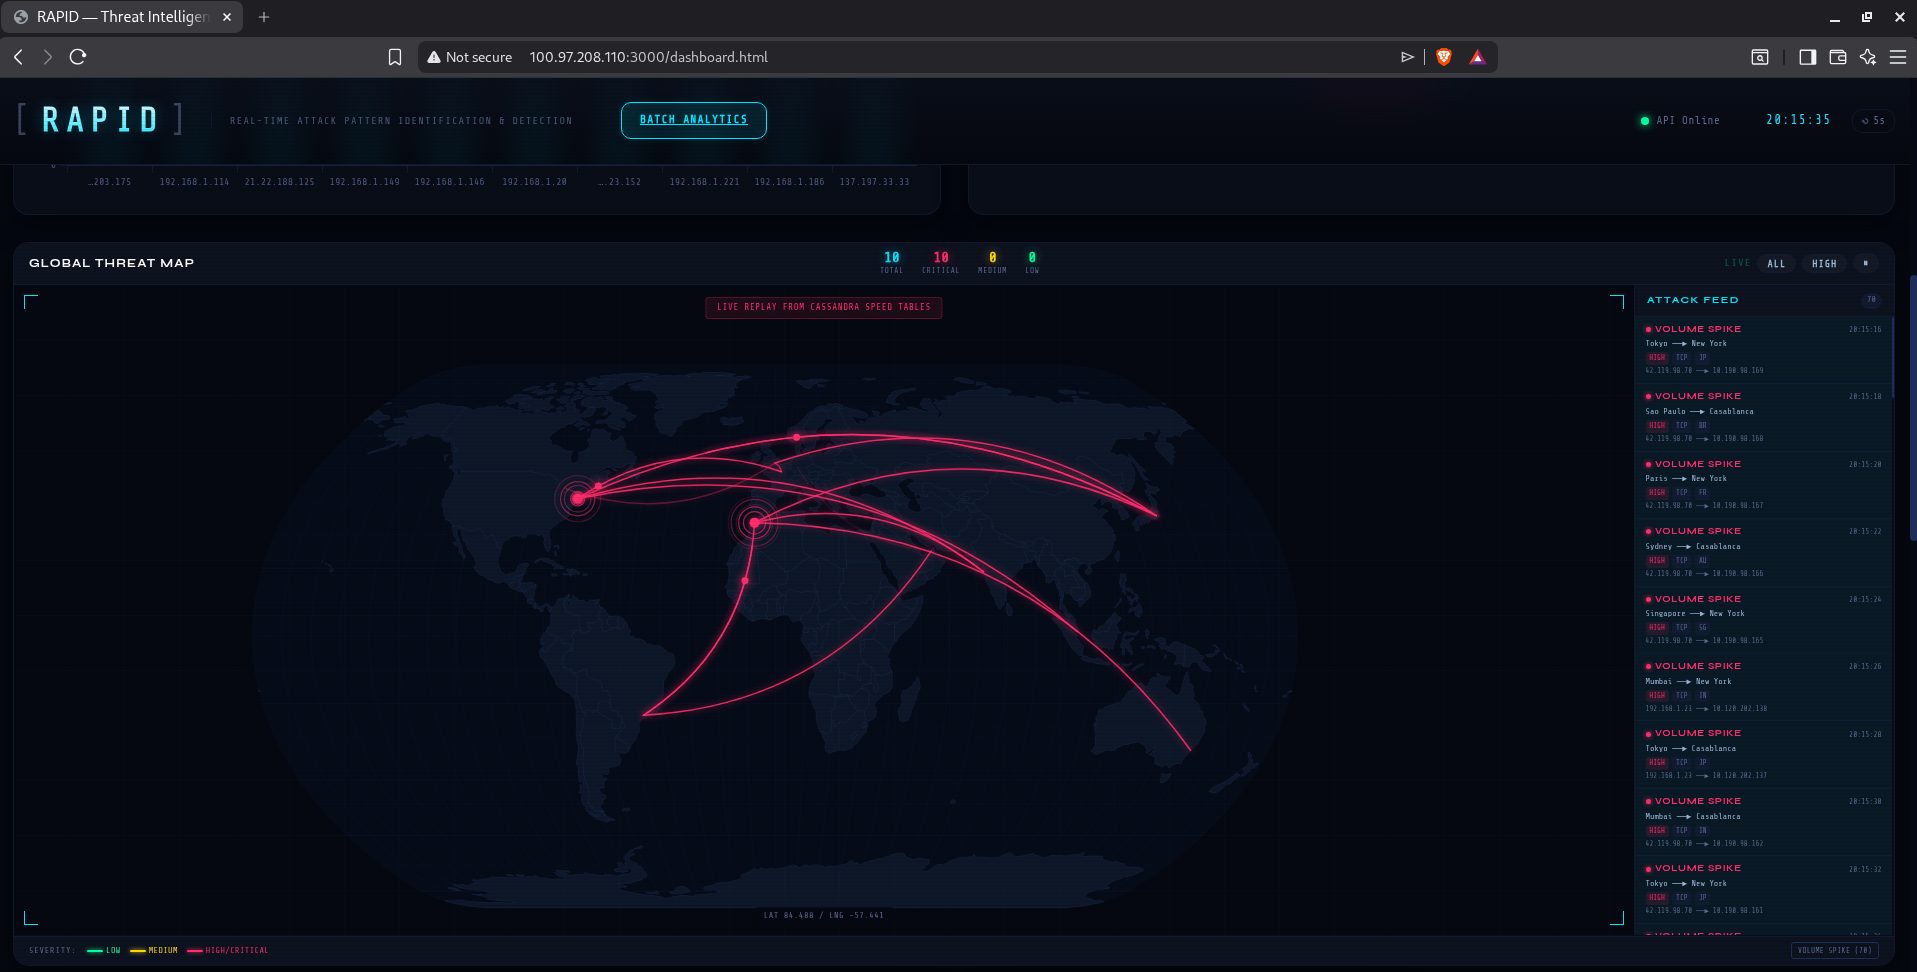
\includegraphics[width=\textwidth]{figures/serving/speed_dashboard/speed_dashboard_global_threat_map.png}
    \caption{Global threat map displaying attack trajectories and the real-time event flow.}
    \label{fig:speed-dashboard-global-map}
\end{figure}

The \textit{Attack Timeline} is a line chart built on the frontend from the scores, volume alerts, signature alerts and real-time threats already loaded. The \textit{Volume Alerts} and \textit{Signature Alerts} tables complement this reading by respectively detailing threshold exceedances and detections associated with signatures.

Figure~\ref{fig:speed-dashboard-timeline-alerts} validates the simultaneous display of the timeline, volume alerts and signature alerts.

\begin{figure}[H]
    \centering
    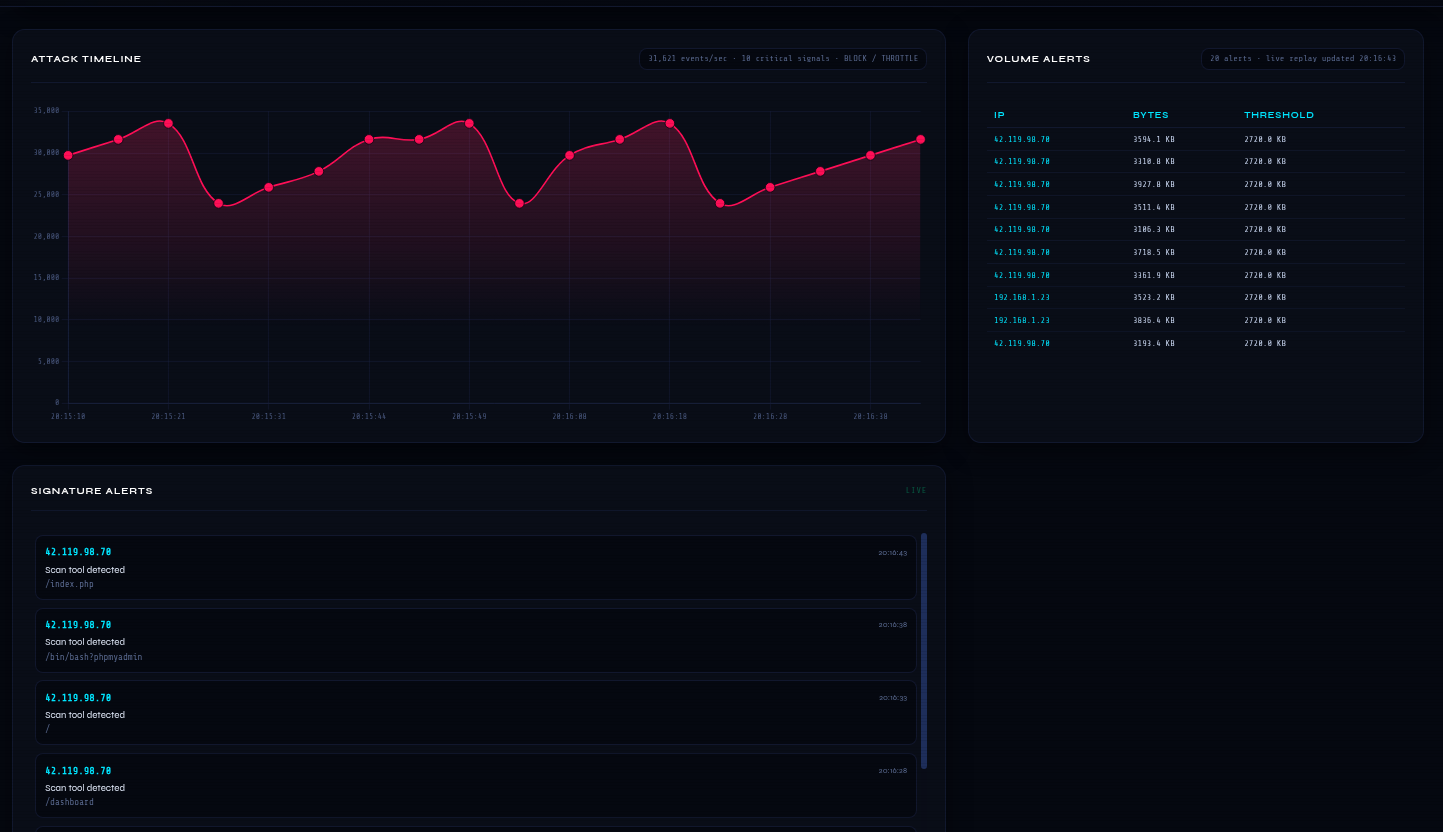
\includegraphics[width=\textwidth]{figures/serving/speed_dashboard/speed_dashboard_timeline_alerts.png}
    \caption{Attack timeline, volume alerts and signature alerts in the real-time view.}
    \label{fig:speed-dashboard-timeline-alerts}
\end{figure}

The \textit{Realtime Decision Queue} aggregates the sources returned by \texttt{/threats/top10?limit=50} and \texttt{/threats/realtime?limit=50}. It organizes IPs according to their score, number of evidences, severity and available consultation action.

This view synthesizes priority sources and facilitates decision-making through the score, number of evidences and severity level.

\begin{figure}[H]
    \centering
    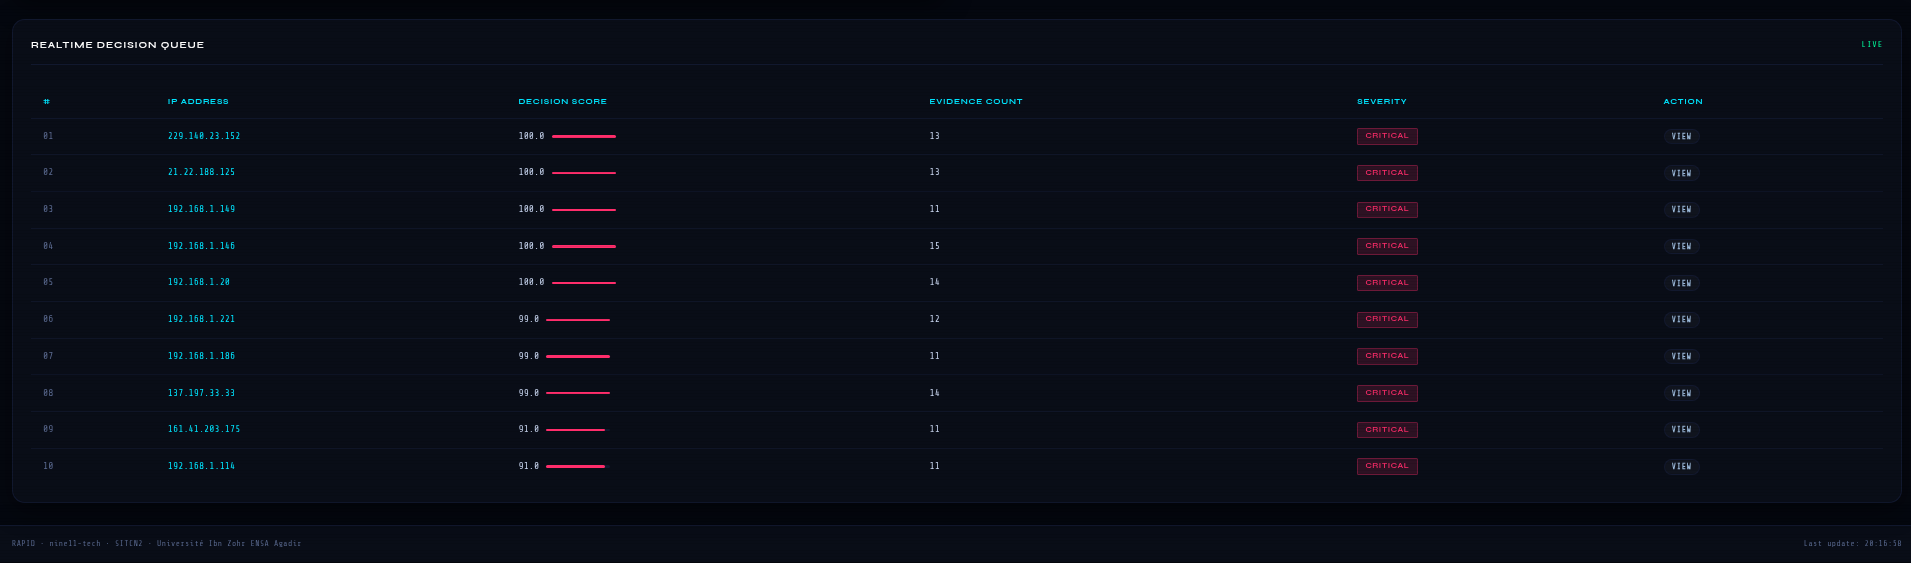
\includegraphics[width=\textwidth]{figures/serving/speed_dashboard/speed_dashboard_decision_queue.png}
    \caption{Real-time decision queue ranking IP addresses by score, evidences and severity.}
    \label{fig:speed-dashboard-decision-queue}
\end{figure}

In the batch view, the \textit{Batch Threat Timeline} chart is a stacked bar chart that represents historical events by day and by threat label. The \textit{Threat Volume} chart compares traffic volumes by category. The \textit{Attack Pattern Types} donut shows the distribution of detected attack families.

This screenshot shows how HBase views are transformed into summary charts: traffic volume by threat class and distribution of attack patterns.

\begin{figure}[H]
    \centering
    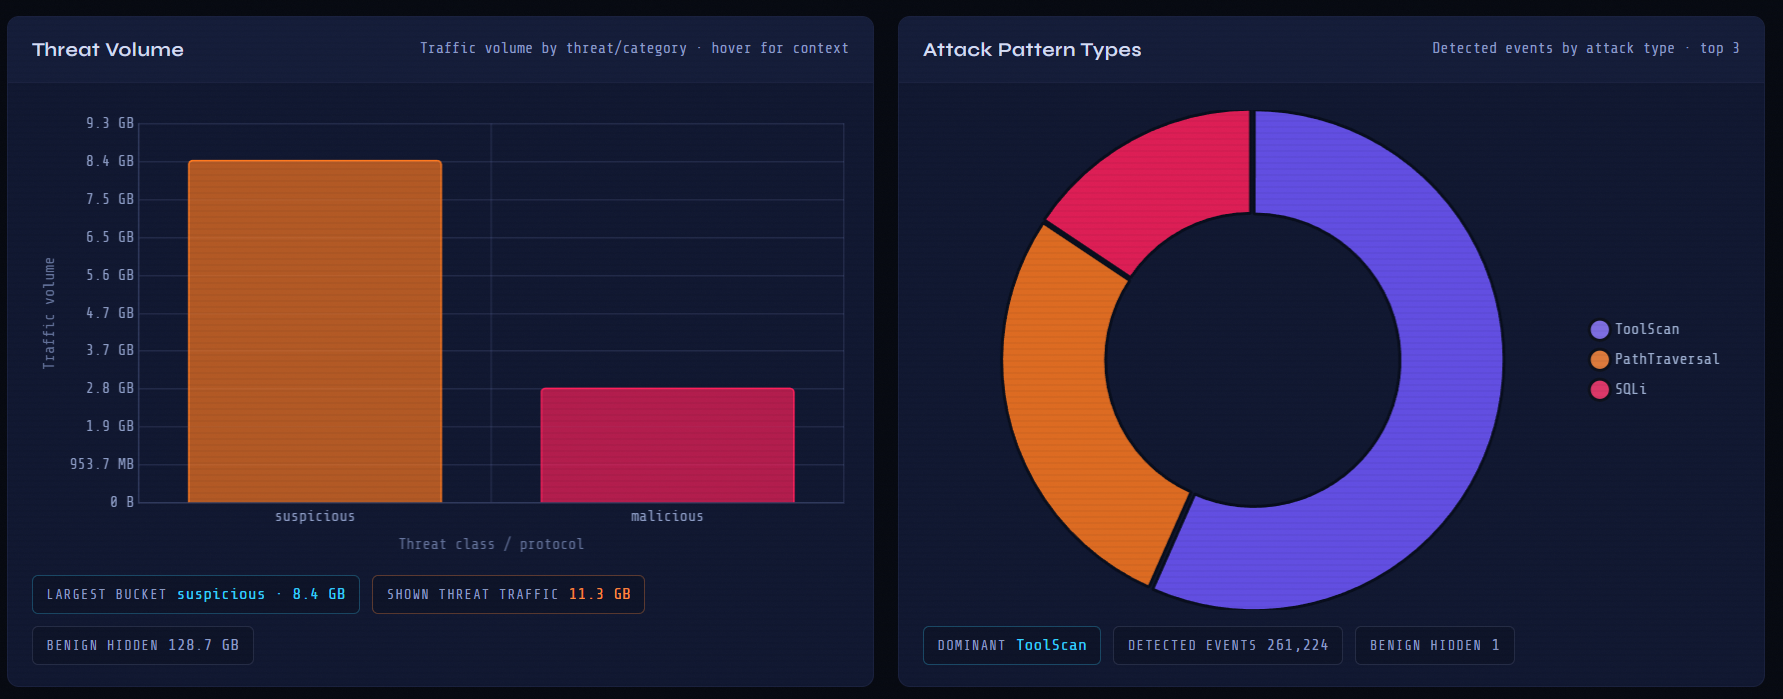
\includegraphics[width=\textwidth]{figures/serving/batch_dashboard/batch_dashboard_volume_patterns.png}
    \caption{Batch charts representing traffic volume by threat category and the distribution of attack families.}
    \label{fig:batch-dashboard-volume-patterns}
\end{figure}

The \textit{IP Reputation Scores -- HBase} chart horizontally ranks IPs according to a decision score recomputed on the frontend from reputation, exploitation indicators and event volume. The \textit{Top Port Scan Sources} chart aggregates scan records by IP and computes a score based on the number of distinct ports, connections and repetition of records.

Figure~\ref{fig:batch-dashboard-portscan-reputation} relates port scan sources to the IP reputation ranking in order to prioritize historical investigations.

\begin{figure}[H]
    \centering
    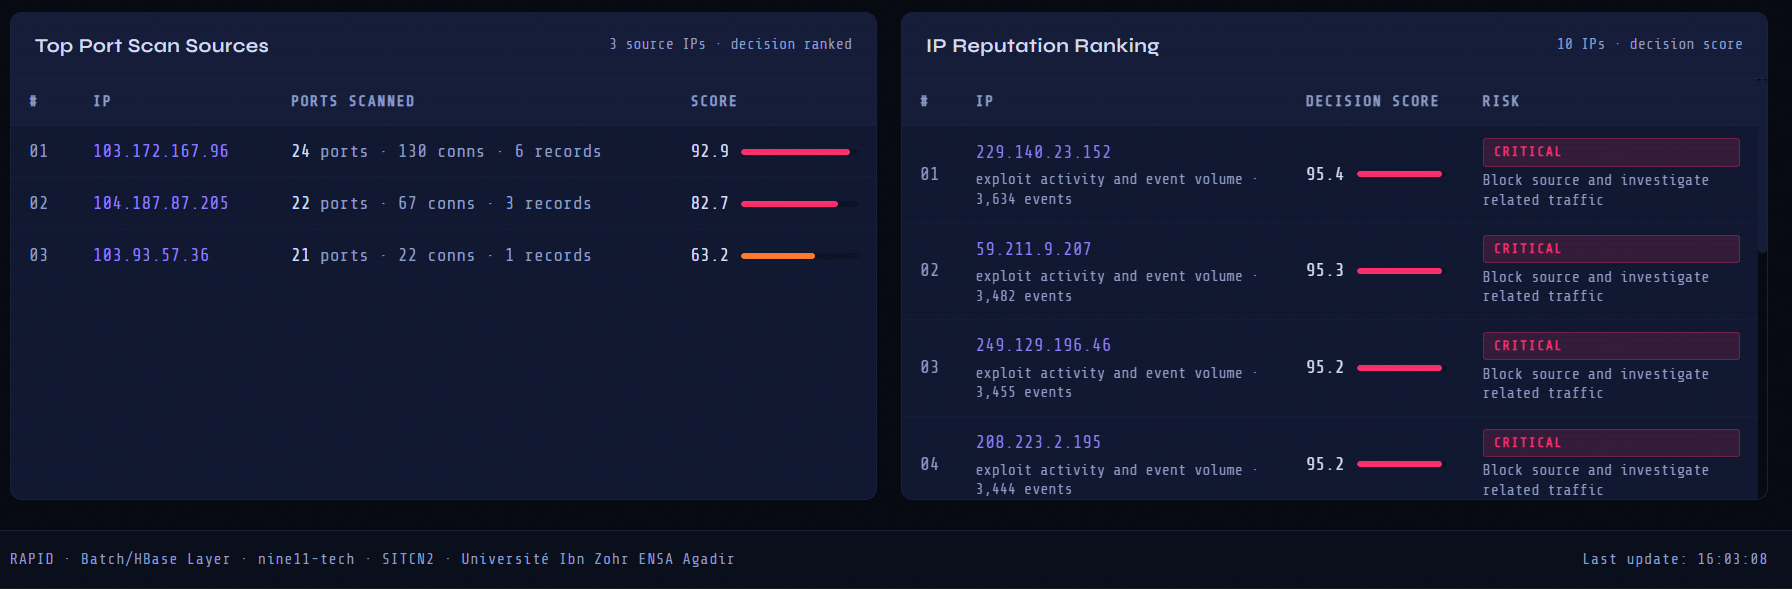
\includegraphics[width=\textwidth]{figures/serving/batch_dashboard/batch_dashboard_portscan_reputation_summary.png}
    \caption{Batch summary of the main port scan sources and the IP address reputation ranking.}
    \label{fig:batch-dashboard-portscan-reputation}
\end{figure}

\begingroup
\scriptsize
\setlength{\tabcolsep}{4pt}
\renewcommand{\arraystretch}{1.30}
\begin{longtable}{|
    >{\raggedright\arraybackslash\bfseries}p{0.23\textwidth}|
    >{\raggedright\arraybackslash}p{0.31\textwidth}|
    >{\raggedright\arraybackslash}p{0.34\textwidth}|
}
    \caption{Summary of dashboard visualizations.}
    \label{tab:dashboard-visualisations}\\
    \hline
    \tablehead{UI Element} & \tablehead{Consumed Data} & \tablehead{Role in the Analysis} \\
    \hline
    \endfirsthead
    \hline
    \tablehead{UI Element} & \tablehead{Consumed Data} & \tablehead{Role in the Analysis} \\
    \hline
    \endhead
    Speed KPI cards & \servingcell{\texttt{/threats/top10}, \texttt{/threats/volume-alerts},\\
    \texttt{/threats/recent}, \texttt{/threats/realtime},\\
    \texttt{/threats/threshold}} & Summarize the activity volume, maximum score, unique IPs, latest activity, adaptive threshold and number of volume alerts. \\
    \hline
    Top Realtime Risk Sources & \servingcell{\texttt{/threats/top10?limit=50}\\
    \texttt{/threats/realtime?limit=50}} & Identify the riskiest source IPs in the speed layer and prioritize decisions. \\
    \hline
    Attack Timeline & \servingcell{Signals already loaded from \texttt{top10}, \texttt{volume-alerts}, \texttt{recent} and \texttt{realtime}} & Represent a synthetic temporal pressure of events and critical signals. \\
    \hline
    Live Detection Mix & \servingcell{Signals already loaded from \texttt{top10}, \texttt{volume-alerts}, \texttt{recent} and \texttt{realtime}} & Show the composition of recent detections: scores, signatures, volume and brute force. \\
    \hline
    Global Threat Map & \servingcell{\texttt{/threats/geo/attacks};\\
    fallback on already loaded speed signals} & Visualize geographic trajectories, severity and attack types in a map flow. \\
    \hline
    Volume Alerts & \servingcell{\texttt{/threats/volume-alerts}\\
    \texttt{?limit=50}} & List IPs that exceed a volume threshold and compare the observed volume with the threshold. \\
    \hline
    Signature Alerts & \servingcell{\texttt{/threats/recent}\\
    \texttt{?limit=50}} & Display alerts derived from signatures, with reason, path or user agent. \\
    \hline
    Realtime Decision Queue & \servingcell{\texttt{/threats/top10?limit=50}\\
    \texttt{/threats/realtime?limit=50}} & Rank IPs by score, number of evidences, severity and consultation action. \\
    \hline
    Batch KPI cards & Main \texttt{/batch/*} endpoints & Count the available historical views: patterns, reputations, scans, multi-step chains, volumes and tables. \\
    \hline
    Batch Threat Timeline & \servingcell{\texttt{/batch/threat-timeline}\\
    \texttt{?limit=50}} & Observe the historical evolution of threats by day and by label. \\
    \hline
    Threat Volume & \servingcell{\texttt{/batch/threat-volume}\\
    \texttt{?limit=10}} & Compare traffic volumes by threat category and identify the largest buckets. \\
    \hline
    Attack Pattern Types & \servingcell{\texttt{/batch/attack-patterns}\\
    \texttt{?limit=30}} & Summarize the distribution of attack families: SQLi, XSS, Path Traversal, ToolScan or other patterns. \\
    \hline
    IP Reputation Ranking & \servingcell{\texttt{/batch/ip-reputation}\\
    \texttt{?limit=30}} & Rank historical IPs according to their reputation score and risk level. \\
    \hline
    Top Port Scan Sources & \servingcell{\texttt{/batch/port-scans/top?limit=10}\\
    \texttt{/batch/port-scans?limit=30}} & Identify the sources that scan the most ports and preserve the associated raw records. \\
    \hline
    Multi-Step Attack Chains & \servingcell{\texttt{/batch/multistep-attacks}\\
    \texttt{?limit=30}} & Highlight IPs that combine several attack stages in the history. \\
    \hline
    Modales de détail IP & \servingcell{\texttt{/threats/ip/}\\\texttt{\textless{}ip\textgreater{}}\\
    batch endpoints by IP} & Group the evidence associated with a source and facilitate the analyst's decision. \\
    \hline
\end{longtable}
\endgroup

This table details the attack patterns extracted from the batch views and makes it possible to identify dominant families, their severity and their decision score.

\begin{figure}[H]
    \centering
    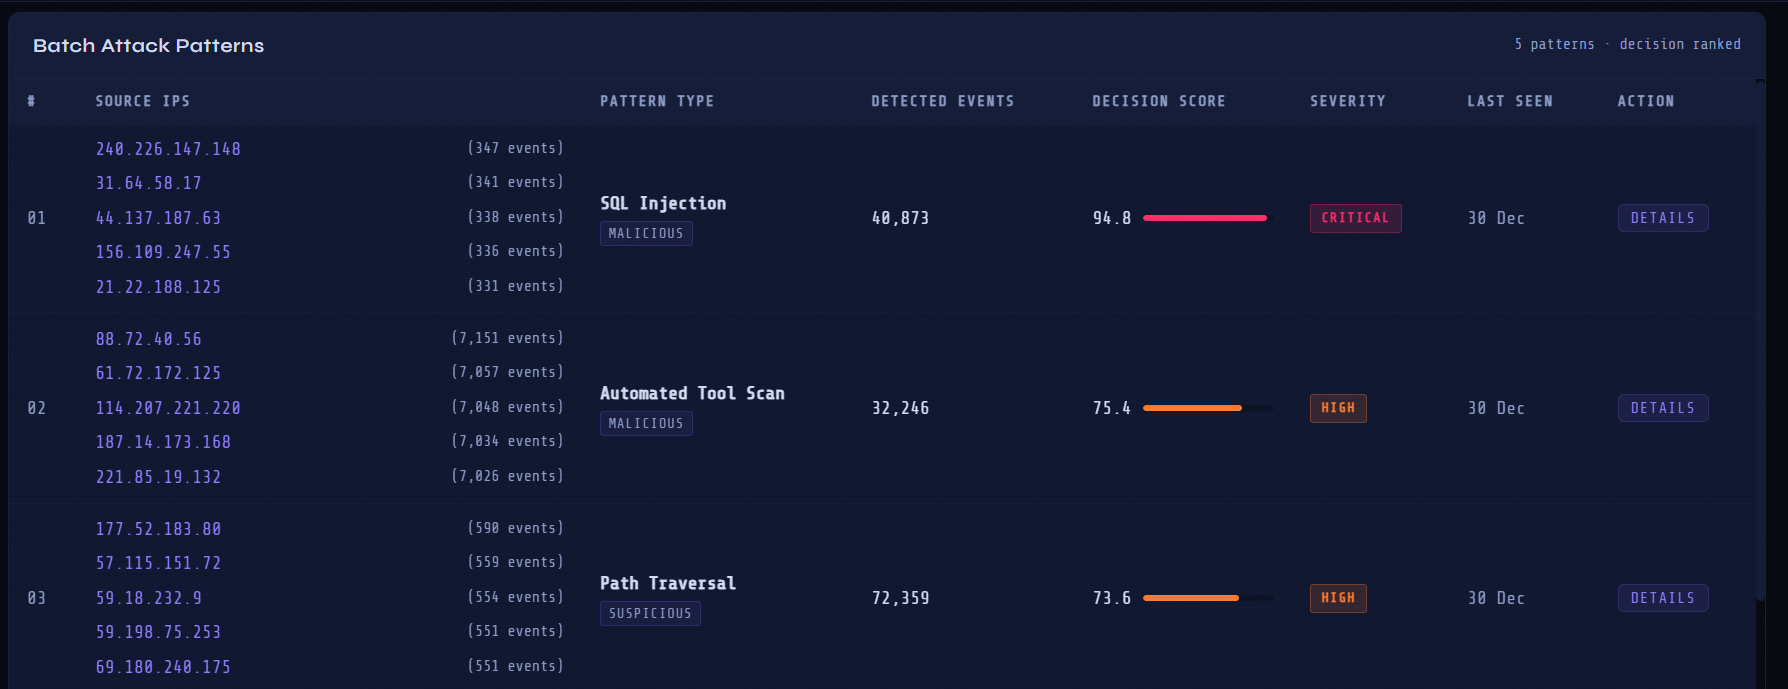
\includegraphics[width=\textwidth]{figures/serving/batch_dashboard/batch_dashboard_attack_patterns_table.png}
    \caption{Batch table detailing attack families, decision scores, severities and latest observations.}
    \label{fig:batch-dashboard-attack-patterns-table}
\end{figure}

The IP reputation table presents the historical scores computed from HBase views and provides direct decision support for the riskiest sources.

\begin{figure}[H]
    \centering
    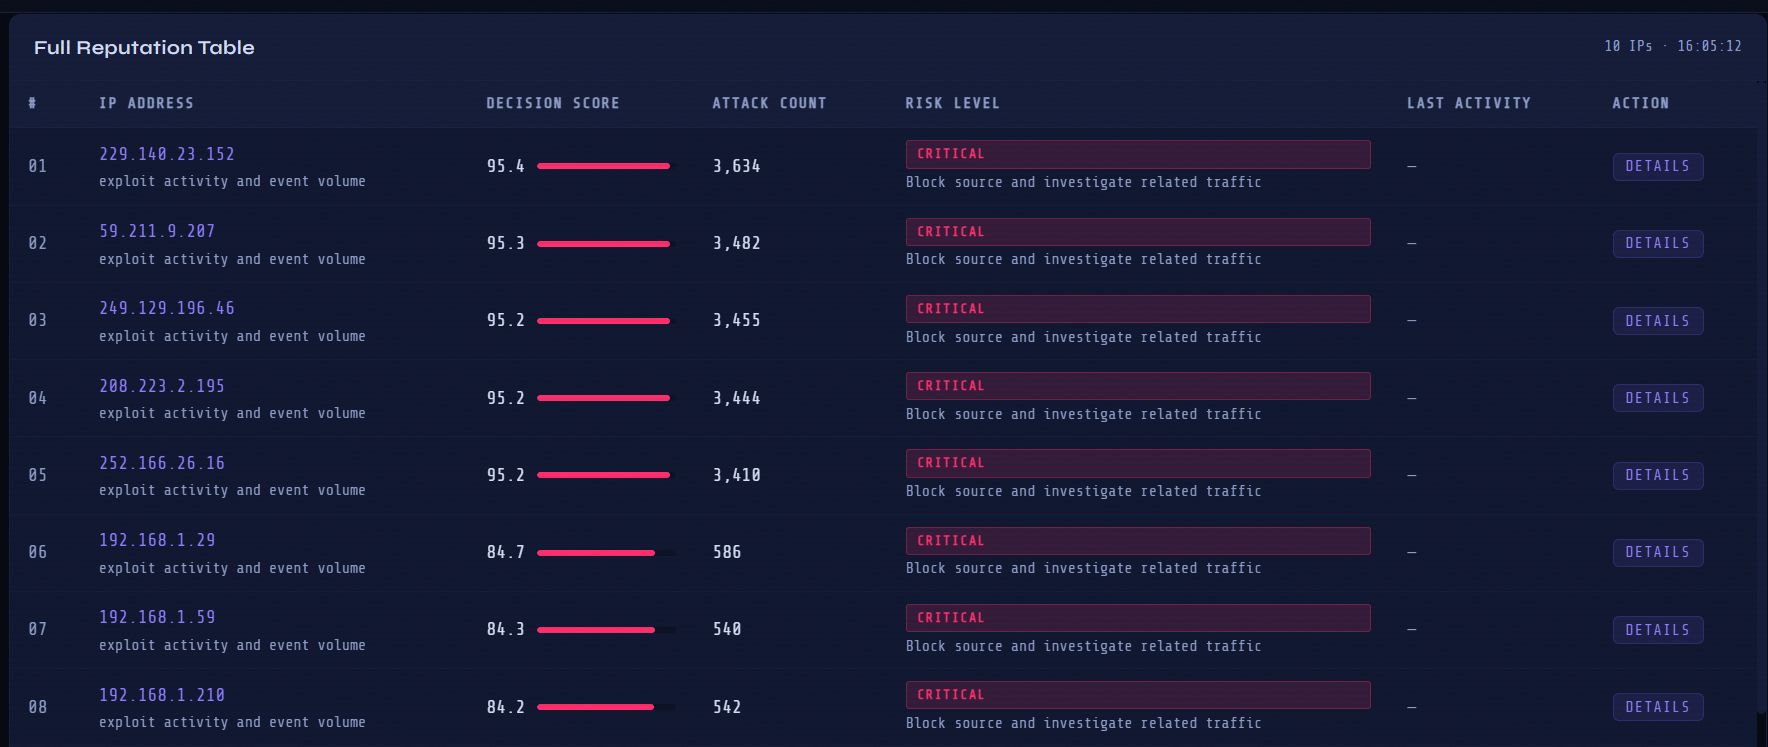
\includegraphics[width=\textwidth]{figures/serving/batch_dashboard/batch_dashboard_ip_reputation_table.png}
    \caption{Complete IP reputation table showing historical scores, risk levels and action recommendations.}
    \label{fig:batch-dashboard-ip-reputation-table}
\end{figure}

This screenshot illustrates detailed port scan records, making it possible to move from an aggregated view to the raw historical observations served by HBase.

\begin{figure}[H]
    \centering
    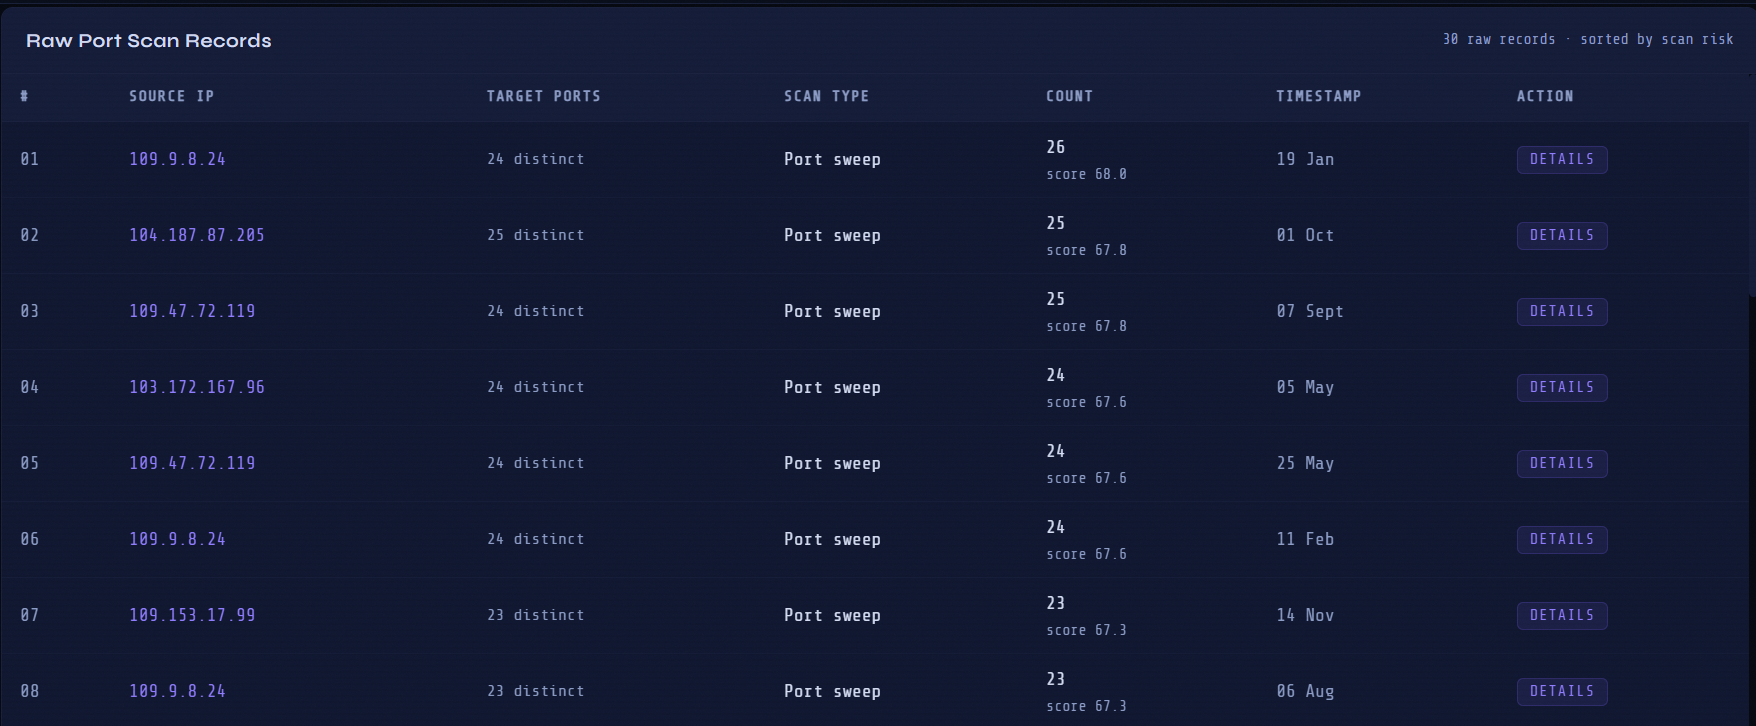
\includegraphics[width=\textwidth]{figures/serving/batch_dashboard/batch_dashboard_raw_port_scan_records.png}
    \caption{Batch port scan records with targeted ports, scan type, counter and observed period.}
    \label{fig:batch-dashboard-raw-port-scans}
\end{figure}

Figure~\ref{fig:batch-dashboard-multistep-chains} shows multi-step correlations, for example ToolScan, then SQLi and Path Traversal, in order to identify structured behaviors on the same IP.

\begin{figure}[H]
    \centering
    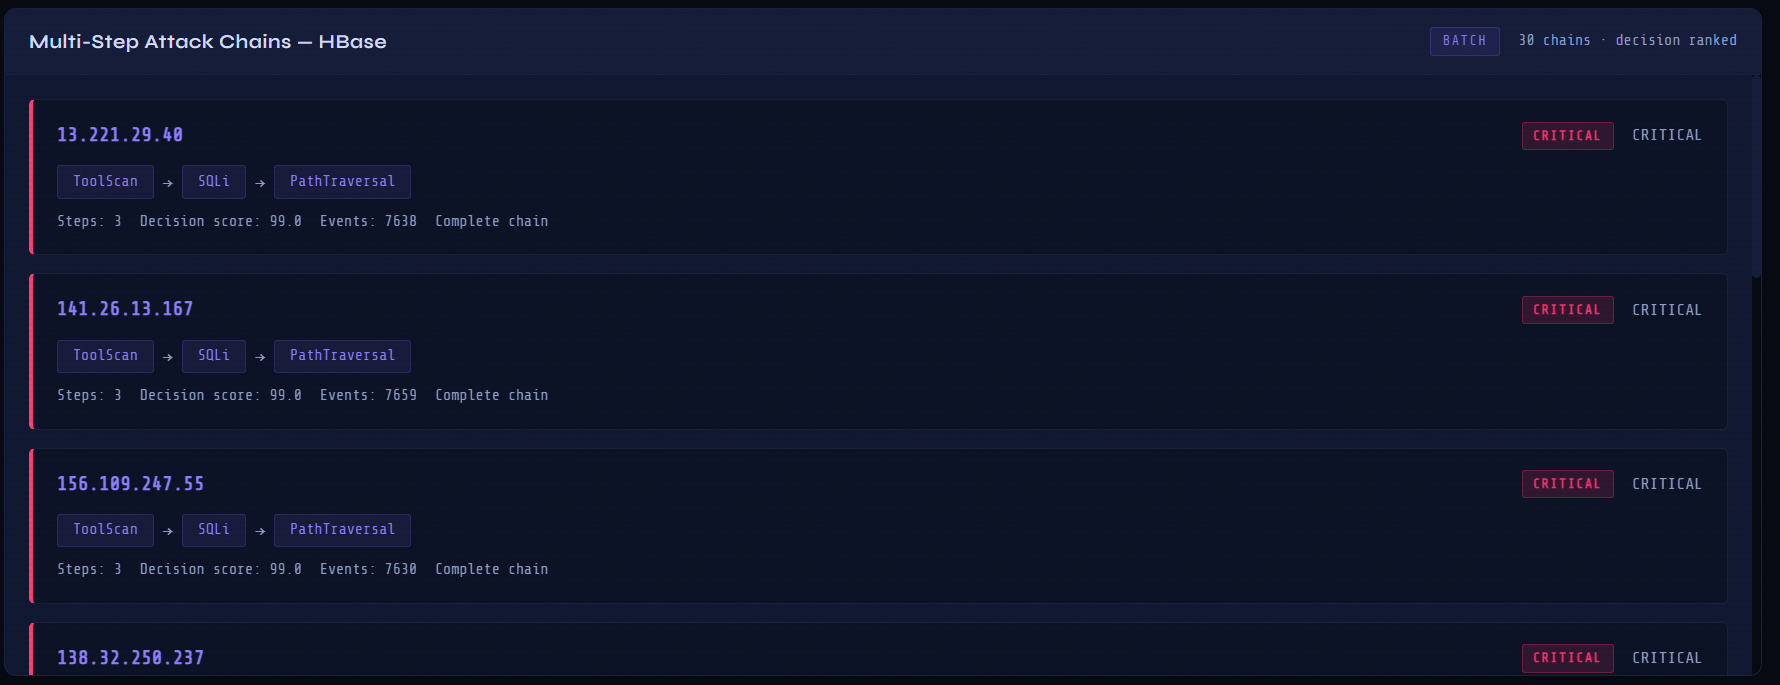
\includegraphics[width=\textwidth]{figures/serving/batch_dashboard/batch_dashboard_multistep_attack_chains.png}
    \caption{Multi-step attack chains detected in HBase with attack sequence, decision score and criticality level.}
    \label{fig:batch-dashboard-multistep-chains}
\end{figure}

\section{Separation between Batch and Speed Views}

The separation between batch and speed remains visible in the frontend, but it does not burden the user with internal computation details. Historical views come from HBase and are displayed in \texttt{batch.html}. They correspond to long-term memory produced by Spark batch processing: IP reputation, attack patterns, timeline, volume, scans and multi-step chains. Real-time results come from Cassandra and are displayed in \texttt{dashboard.html}. They represent the recent operational state: scores, signature alerts, volume alerts, active threats and adaptive threshold.

The dashboard merges these two perspectives at the user experience level. An IP can be studied from the speed view with \texttt{/threats/ip/<ip>}, which exposes both the recent state and a historical score. It can also be studied from the batch view with the HBase endpoints specific to the IP. In both cases, the frontend consumes already structured API responses. It does not need to know the Spark steps, the exact Cassandra tables, or the HBase scans performed by the backend. This separation respects the principle of the Lambda Architecture: the batch layer provides historical depth, the speed layer provides freshness, and the serving layer presents both in an exploitable form.

\section{Visual Validation of the Dashboard}

The screenshots integrated into this chapter validate the two temporalities of the serving layer. The speed views show the real-time indicators from Cassandra, the global map, the timeline, the alerts and the decision queue. The batch views show the historical results served from HBase: batch timeline, volumes, attack patterns, IP reputation, port scans and multi-step chains. This visual validation confirms that the results computed by the batch and speed layers are effectively accessible in the final interface.

\section{Chawi's Contribution to the Serving Layer}

Chawi's contribution in this layer concerns the final availability of analytical results. It includes the static dashboard, the visual presentation of results, the connection between API responses and HTML/JS components, and the hosting of the interface in the \texttt{chawi} profile with the \texttt{nginx-dashboard} container. This responsibility complements his role on HBase and Cassandra: the data are not only stored in NoSQL databases, they become queryable through an interface ready for demonstration.

More precisely, Chawi ensures the presentation part of the serving layer. The \texttt{batch.html}, \texttt{dashboard.html}, \texttt{batch.js}, \texttt{main.js}, \texttt{batch.css} and \texttt{style.css} files define the structure, charts, statistic cards, tables and modals. JavaScript transforms JSON responses into visible components: KPI values, score bars, severity badges, alert feeds, sorted tables and Chart.js charts. This contribution connects the results of the Lambda Architecture to an operational reading understandable by an analyst.

\section{Summary}

The RAPID serving layer transforms the technical outputs of the pipeline into an analysis interface. HBase provides the historical batch views, Cassandra provides the recent speed results, Flask exposes the REST endpoints, and the HTML/JavaScript dashboard displays information as cards, charts, tables, alerts and interactive maps. This organization keeps the frontend simple: it consumes API responses and updates the DOM, without carrying the details of Spark processing or NoSQL queries.

The dashboard therefore fulfills an essential function in the project. It verifies that the results are not only computed, but also served and interpretable. The separation between \texttt{batch.html} and \texttt{dashboard.html} makes the historical/real-time duality explicit, while IP searches and detail modals bring these two temporalities together at decision time.
